% !TEX root = ../../../main.tex
% 来源：中学数学实验教材·第三册（高中数学）
% 章节：任意角的三角函数 / 弧和角的概念及其度量
% 原始文件：6.tex，行 164-178
% 类型：tikz
% ---
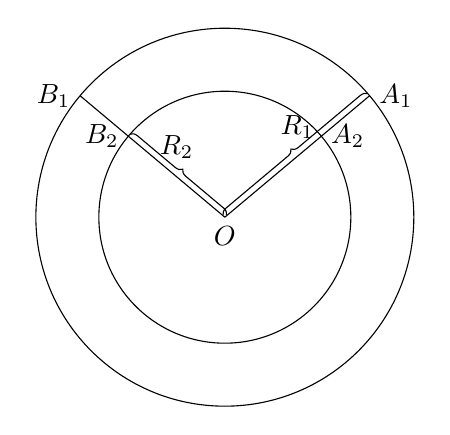
\begin{tikzpicture}[scale=.8]
\draw (0,0) circle (2);
\draw (0,0) circle (3);
\draw (0,0)--(40:3);
\draw (0,0)--(140:3);

\node at (40:2)[right]{$A_2$};
\node at (40:3)[right]{$A_1$};
\node at (140:2)[left]{$B_2$};
\node at (140:3)[left]{$B_1$};
\node at (0,0)[below]{$O$};

\draw[decorate,decoration={brace,raise=1pt}] (0,0)--node[above=3pt]{$R_1$}(40:3);
\draw[decorate,decoration={brace,raise=1pt}] (140:2)--node[above=3pt]{$R_2$}(0,0);
\end{tikzpicture}
